\chapter{Test \& Analysis}
\label{chap:test}

This chapter is divided into 2 parts. 
The first part is for requirements testing, where experiments are conducted to evaluate whether all four requirements of the coursework have been successfully implemented.
The second part is for network performance testing, where experiments are conducted to evaluate the performance of the whole network.
In addition, the effects of data acknowledgements on the performance are analyzed.

\section{Requirements Testing}

For requirements testing, all 6 nodes are included. 
As detailed in Section \ref{sec:architecture}, one node acts as the source device, one as the destination device, and the others as intermediate nodes.

Figure \ref{fig:test-req} shows the position of all six nodes in the network. 
The source device is placed on the leftmost side, the destination device on the rightmost side, and the intermediate nodes in the middle.

\begin{figure}
\centering
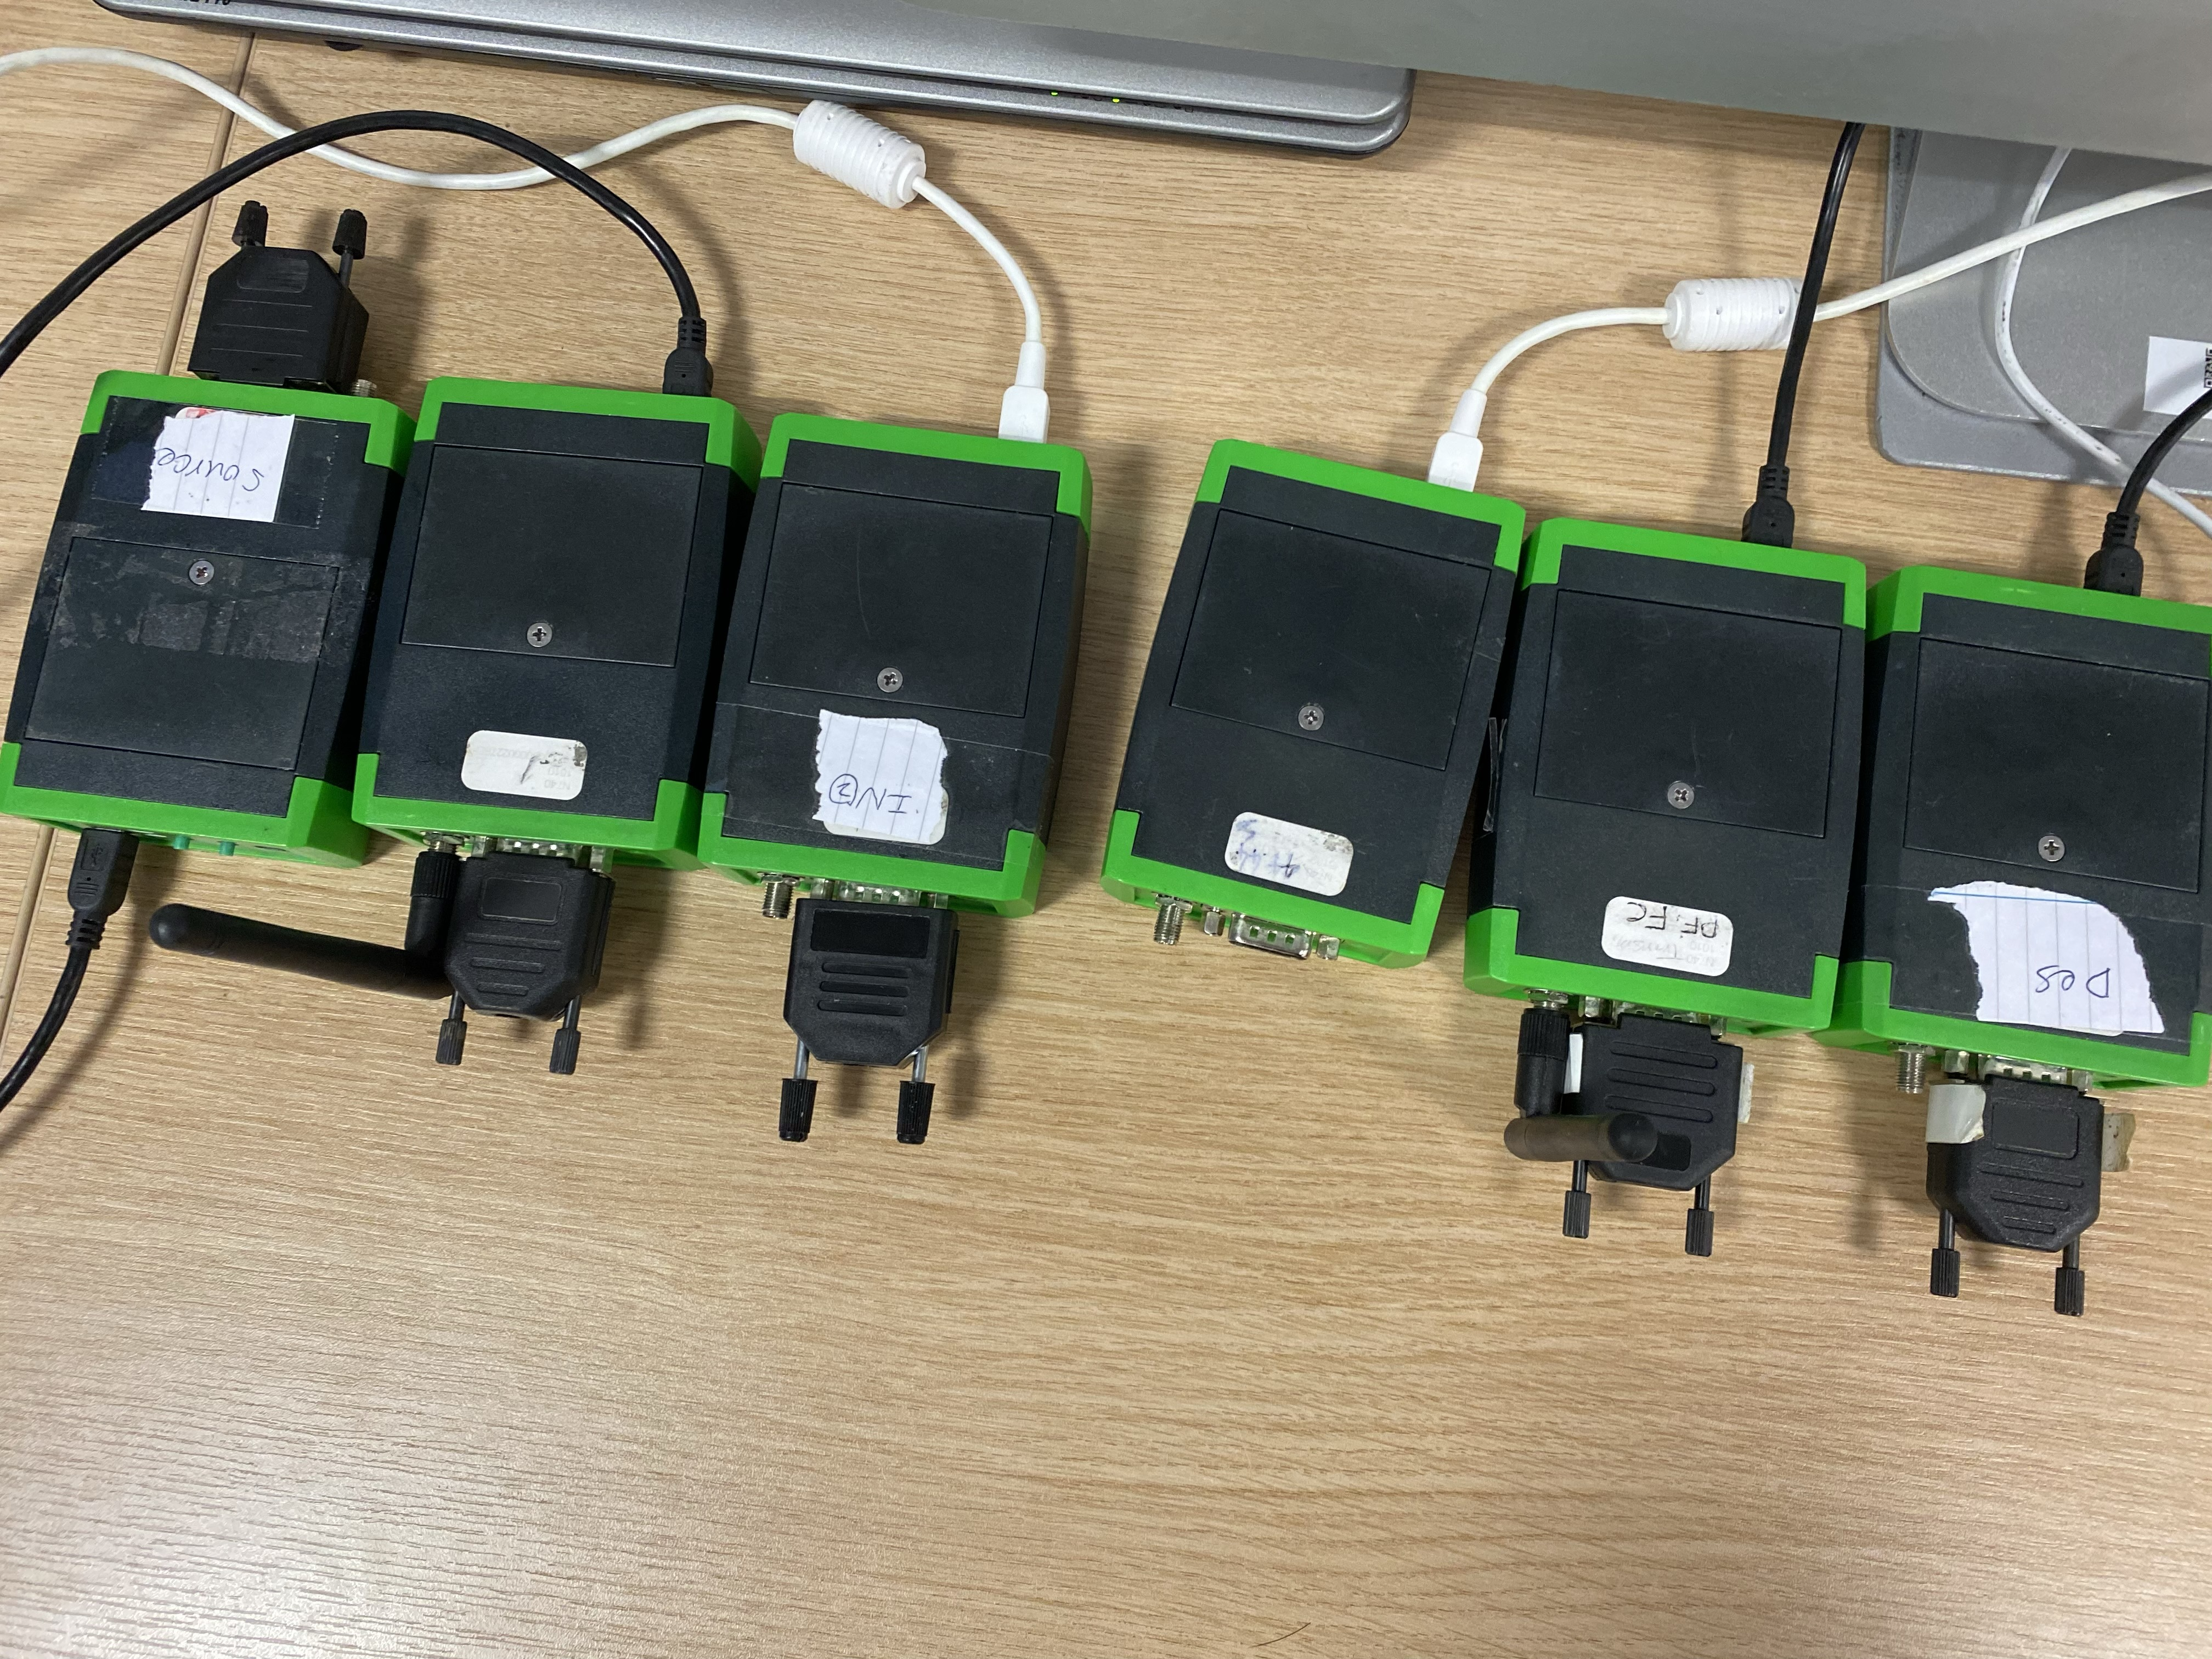
\includegraphics[width=0.7\textwidth]{test-req}
\caption{Position of All Six Nodes in the Network.}
\label{fig:test-req}
\end{figure}

Each node is assigned with a unique MAC address within the group. The source device is assigned with address of AA:AA (170:170), while the destination device is DF:DF (223:223).
The remaining intermediate nodes are assigned with addresses of 01:01, 02:02, 03:03 and 04:04 respectively.


\subsection{Requirement 1 \& 3: Regular Sensors and Route Reporting on Destination Node}

\subsubsection{Experiment Steps}

All devices are turned on. Button 1 on the source device is pressed to initiate regular sensors reporting.

\subsubsection{Expected Results}
The source device should first initiate a route discovery request (RREQ) towards the destination device.
Once it receives a route discovery reply (RREP) and inserts a route, it should send out a data packets using the learned route per 2 second.

If the learned route is valid, the destination device should receive the data packet and send back an acknowledgement.

If the learned route is invalid (eg. weak signal, changes of position), the destination device would not receive the data packet and not send back an acknowledgement.
In that case, the source device would not get an acknowledgement and should initiate a route discovery request again and stop sending out data packets until a new route is learned.

\subsubsection{Results}
Figure \ref{fig:test-1-source} shows the output from the source device.
Once the button is pressed, the source device initiates a route discovery request towards 223.223, which is the destination device.
A reply is received directly from the destination and a new route is thus learned, of which the route index is $-78.0$.

\begin{figure}
\centering
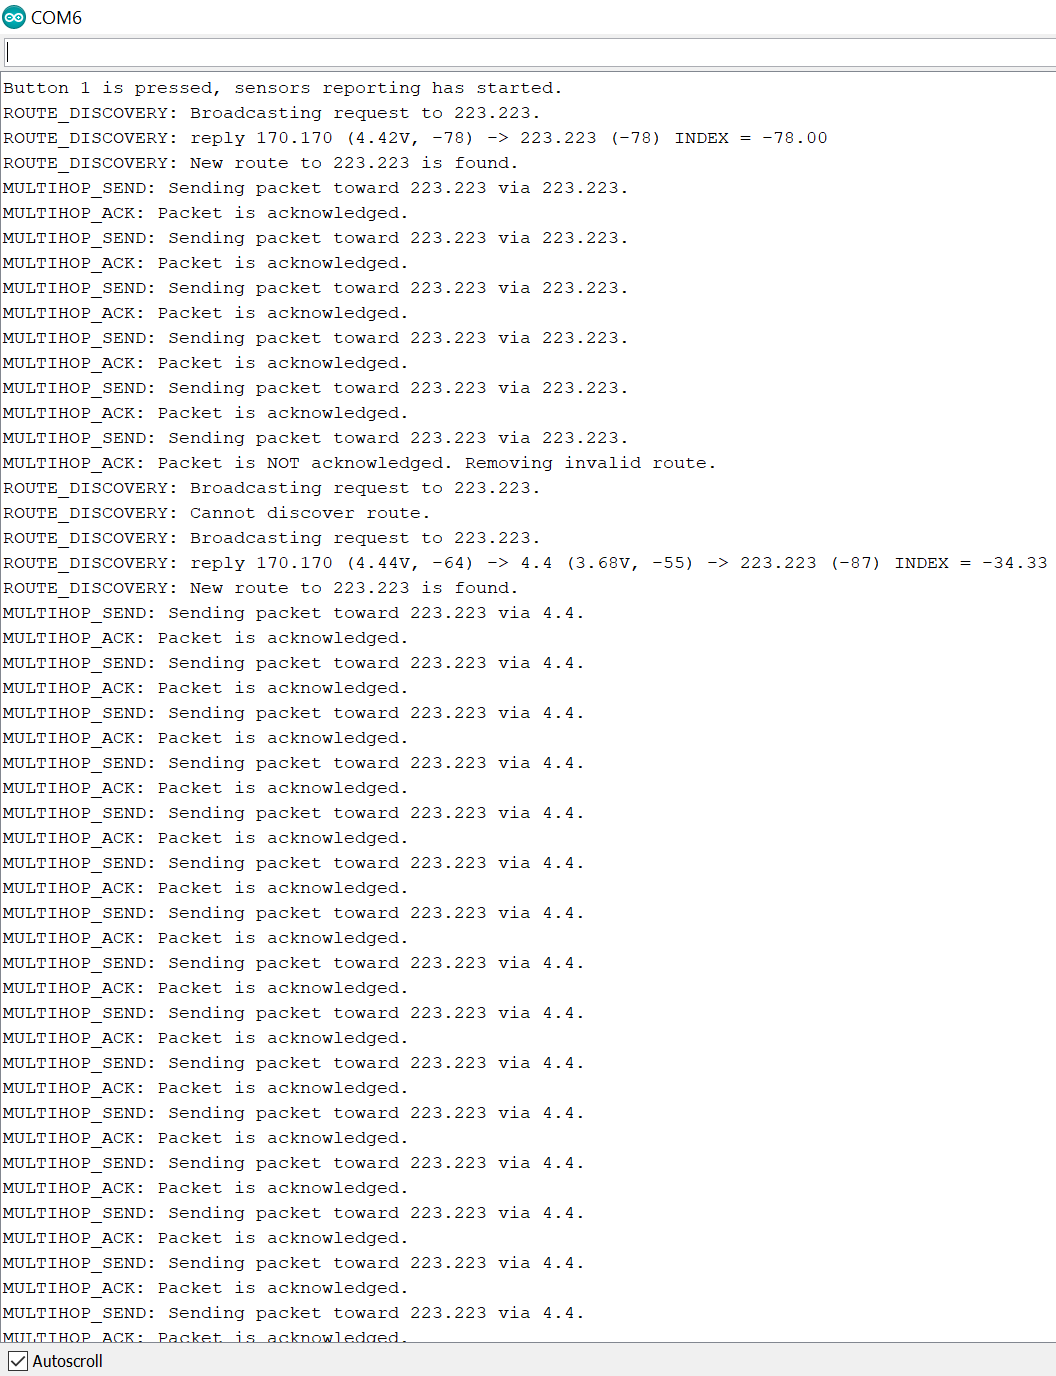
\includegraphics[width=0.7\textwidth]{test-1-source}
\caption{Output from the Source Device After Regular Sensors Reporting Is Started.}
\label{fig:test-1-source}
\end{figure}

The source device starts sending out sensors reading regularly towards the destination device through the route.

On the sixth data packet, an acknowledgement is not received. The source perceives that the route is no longer valid and initiates a route discovery request towards 223.223 again.
A reply is later received from 4:4, which is the fourth intermediate node, and a new route towards the destination is thus learned, of which the route index is $-34.33$.

The source device starts sending out sensors reading regularly towards the destination device through the route again.

Figure \ref{fig:test-1-dest} shows the output from the destination device.
The destination device first receives route discovery request (RREQ) from 170:170, which is the source device and sends back an reply (RREP).
It later receives and displays six data packets from the source, all of which include temperature and battery reading from the source device.
In addition, the data packets include the route each packet take from the source to the destination.

\begin{figure}
\centering
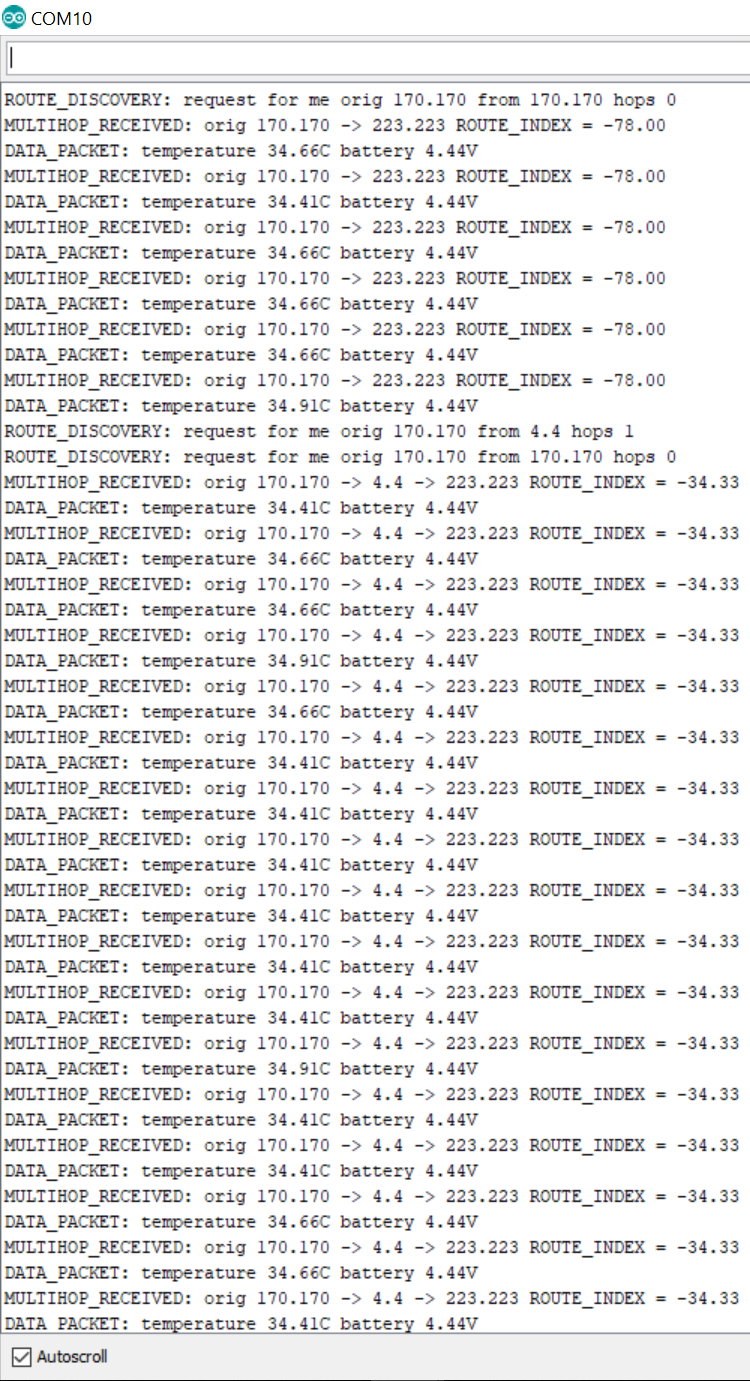
\includegraphics[width=0.7\textwidth]{test-1-dest}
\caption{Output from the Destination Device After  Regular Sensors Reporting Is Started.}
\label{fig:test-1-dest}
\end{figure}

Two new RREQ are then received since the source perceives that the previous direct route is no longer valid and initiates new route discovery requests.
After the new route through 4:4 is established, the destination device starts receiving data packets from the source again.


\subsection{Requirement 2: On-Demand Sensors Switching on Source Node}

\subsubsection{Experiment Steps}
All devices are turned on. 
Button 1 on the source device is pressed to initiate regular sensors reporting.
After a while, Button 2 on the source device is pressed to switch from temperature reporting to light reporting.

\subsubsection{Expected Results}
Once Button 2 is pressed, the source device should switch from temperature reporting to light reporting, or from light reporting to temperature reporting.



\subsubsection{Results}

Figure \ref{fig:test-2-source} shows the output from the source device.
The source device first sends out data packets towards the destination (223:223) through the fourth intermediate node (4:4).
The source device, on receiving that Button 2 is pressed, switches to reporting light sensors reading. 

\begin{figure}
\centering
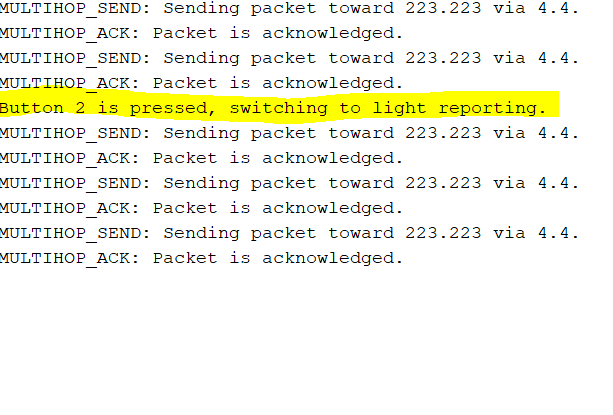
\includegraphics[width=0.7\textwidth]{test-2-source}
\caption{Output from the Source Device After Sensors Reporting Is Switched.}
\label{fig:test-2-source}
\end{figure}

Figure \ref{fig:test-2-dest} shows the output from the destination device.
The destination device first receives data packets that contain temperature and battery voltage readings.
After Button 2 on the source device is pressed, it starts receiving data packets that contain light and battery voltage readings.

\begin{figure}
\centering
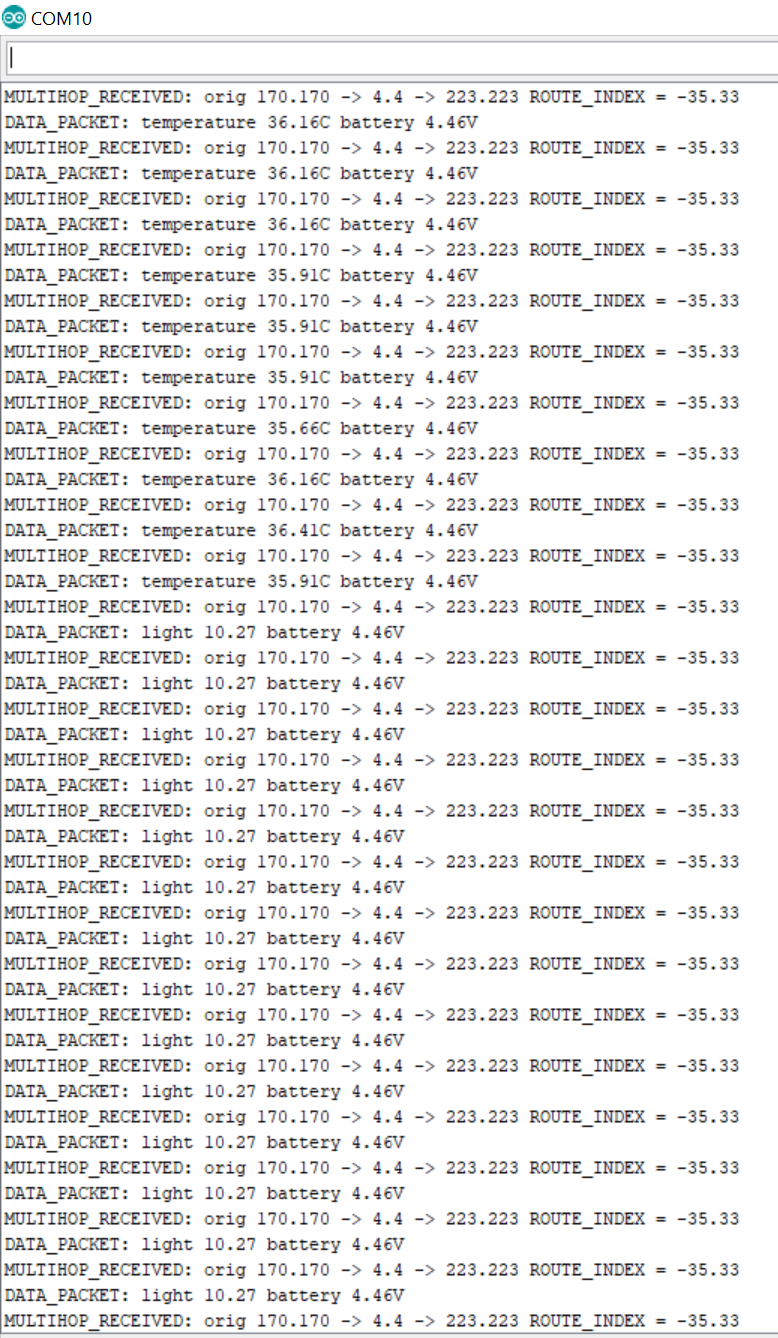
\includegraphics[width=0.7\textwidth]{test-2-dest}
\caption{Output from the Destination Device After Sensors Reporting Is Switched.}
\label{fig:test-2-dest}
\end{figure}

\subsection{Requirement 4: Dynamic Routing}

In this test, sudden changes of intermediate nodes are introduced in the middle of the data delivery by switching off some of intermediate nodes.
According the requirement, one should expect that the source device learns of the lost of intermediate nodes and learns a new route right away.

\subsubsection{Experiment Steps}
All devices are turned on.
Button 1 on the source device is pressed to initiate regular sensors reporting.
After a stable non-direct route is established between the source and the destination, one of the intermediate nodes on the route is switched off.

\subsubsection{Expected Results}
After one of the intermediate nodes on the route is switched off, the source device will no longer be able to send data packets to the destination using the previously learned route.
It receives no acknowledgement from the destination and should then perceive that the route is no longer valid.
The source is expected to initiate a new route discovery request (RREQ) to learn a new route.

\subsubsection{Results}

Figure \ref{fig:test-4-source} shows the output from the source device.
At first, the source device learns a route towards the destination through the fourth intermediate node (4:4).
After the fourth intermediate node is switched off manually, the source device receives no acknowledgement for the last data packet it sends.
It removes the route from its route table and initiates a new route request towards the destination.

\begin{figure}
\centering
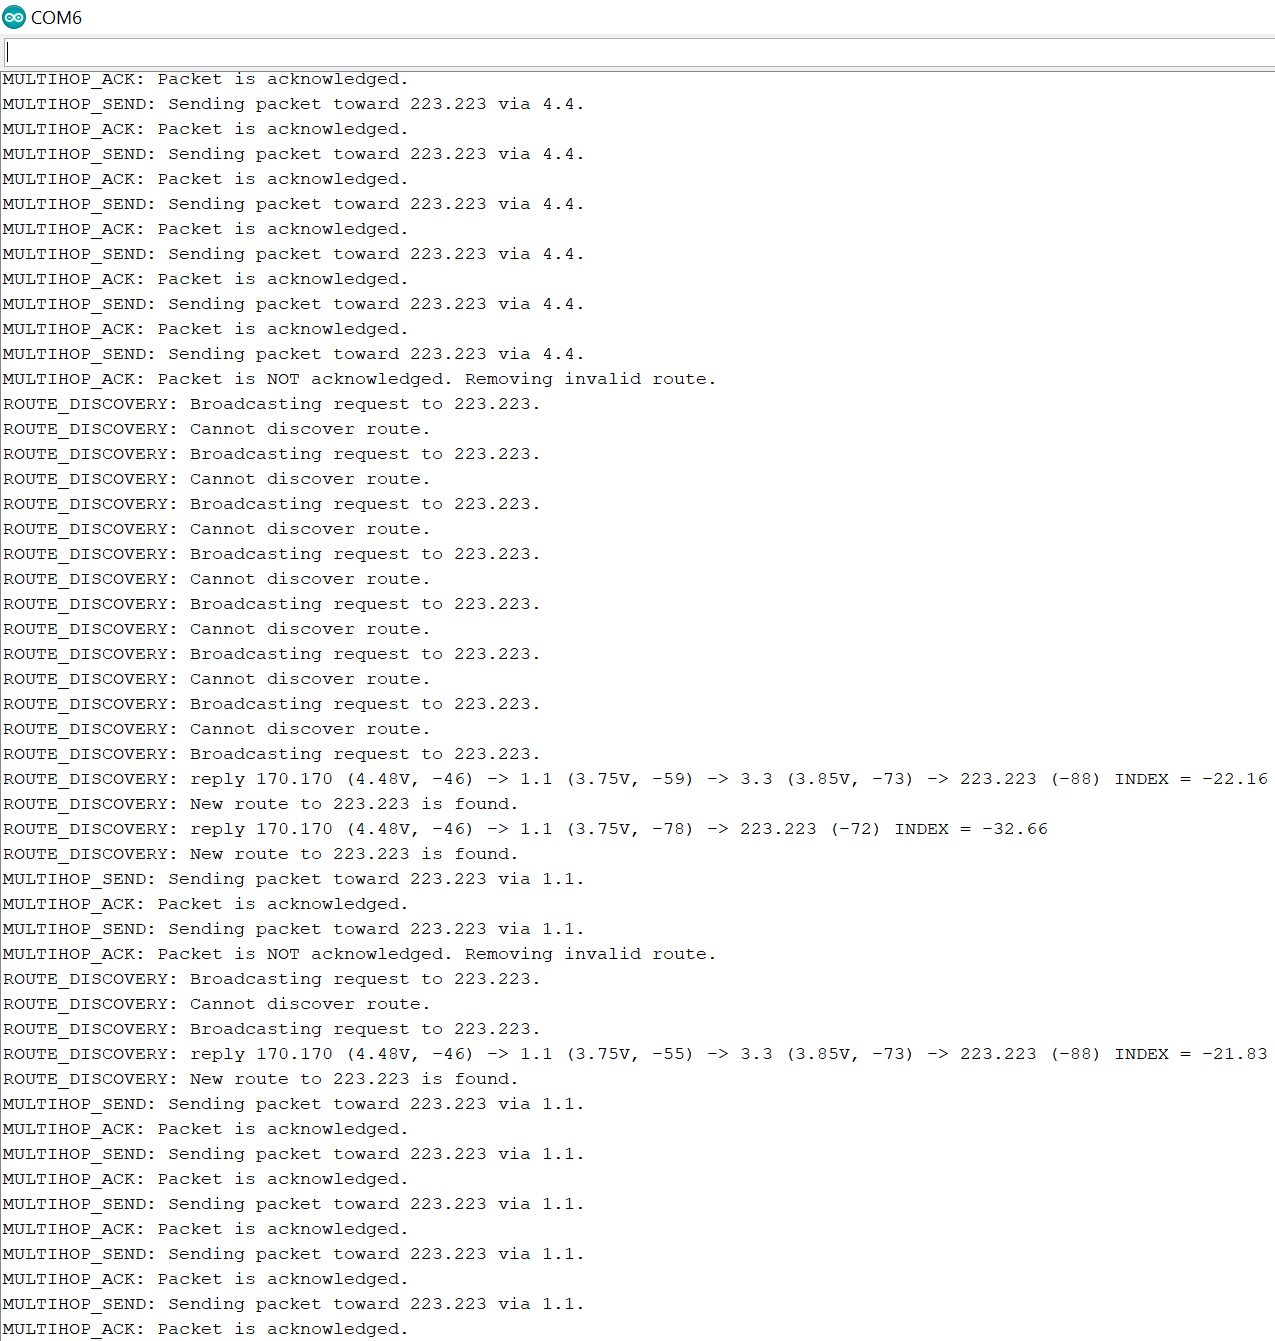
\includegraphics[width=0.7\textwidth]{test-4-source}
\caption{Output from the Source Device After Changes of Intermediate Nodes in the Network.}
\label{fig:test-4-source}
\end{figure}


After a few trials, the source learns a stable route towards the destination through the first intermediate node (1:1) and later the third intermediate node (3:3).
It sends data packets to and receives acknowledgements from the destination regularly.

Figure \ref{fig:test-4-dest} shows the output from the destination device.
It first receives sensors reading from the source through the fourth intermediate node (4:4). 

\begin{figure}
\centering
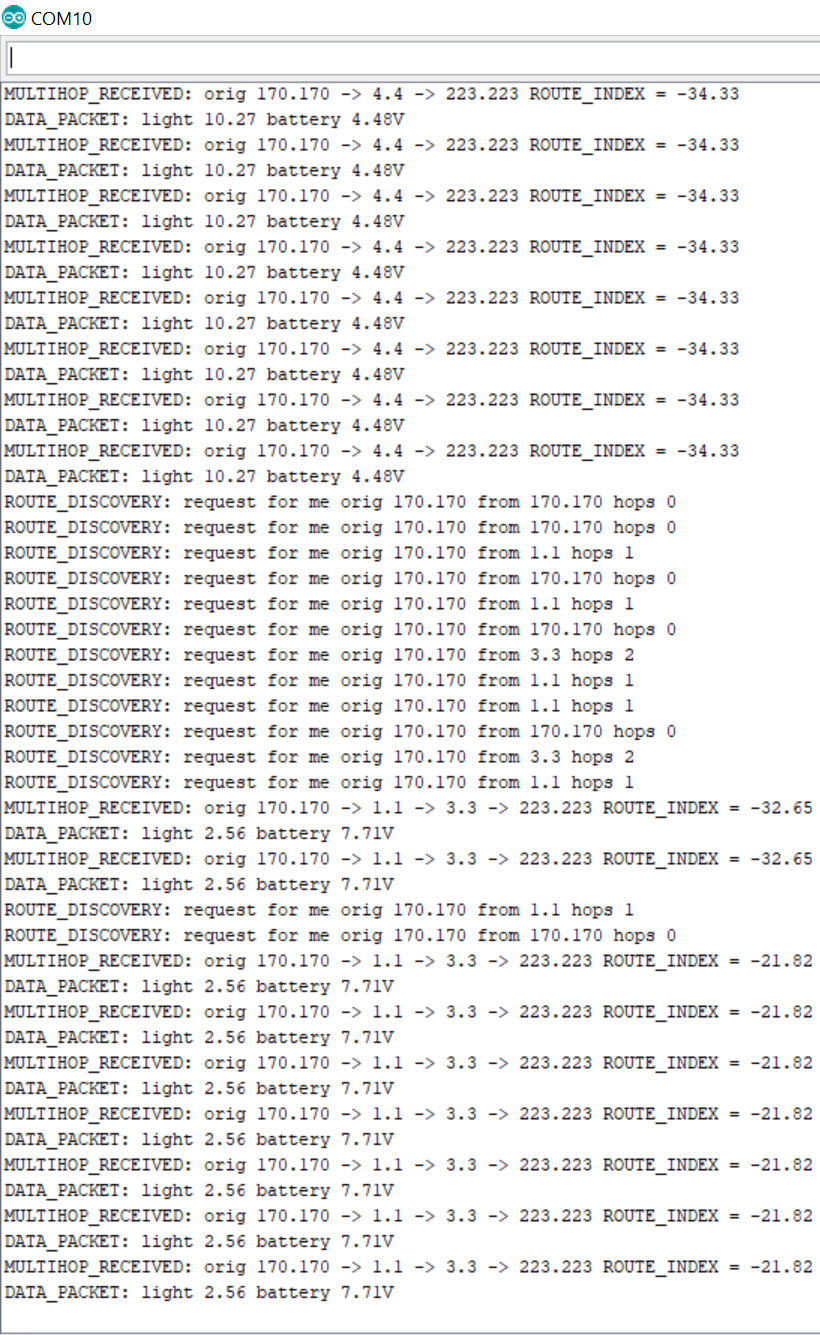
\includegraphics[width=0.7\textwidth]{test-4-dest}
\caption{Output from the Destination Device After Changes of Intermediate Nodes in the Network.}
\label{fig:test-4-dest}
\end{figure}

After the fourth node is switched off, it receives several RREQ from the source when the source is requesting a route to it.
After the source learns a stable route towards the destination, the destination device starts regularly receiving data packets from the source device through the new route.
The new route goes through the first intermediate node (1:1) and later the third intermediate node (3:3).

